%%%%%%%%%%%%%%%%%%%%%%%%%%%%%%%%%%%%%%%%%%%%%%%%%%%%%%%%%%%%%%%%%%%%%%%%
%%% New Section 3.1: Belief-Conditioned Program Games (Symmetric)
%%% 
%%% This is a rewrite of Section 3.1 from DiGiovanni, Clifton, and 
%%% Macé (2024), "Safe Pareto Improvements for Expected Utility 
%%% Maximizers in Program Games," extending the program game framework 
%%% to allow for:
%%%   (1) Conditional beliefs: each player i's beliefs about j's 
%%%       program depend on i's own program choice (symmetric partial 
%%%       prediction / acausal influence).
%%%   (2) Belief-conditioned programs: programs take the other player's
%%%       conditional belief function as input, in addition to the 
%%%       other player's program.
%%%
%%% Written in the style of the original Section 3.1, as for a 
%%% follow-up paper citing the original.
%%%%%%%%%%%%%%%%%%%%%%%%%%%%%%%%%%%%%%%%%%%%%%%%%%%%%%%%%%%%%%%%%%%%%%%%

\documentclass[sigconf]{aamas} 
\usepackage{defaults}

\usepackage{thm-restate}


\newcommand{\epsdeltaone}{\epsilon_1}
\newcommand{\bestparetopayoffi}{u^*_i}
\newcommand{\bestparetopayoffj}{u^*_j}
\newcommand{\bestparetopayoffone}{u^*_1}
\newcommand{\bestparetopayofftwo}{u^*_2}
% \newcommand{\pmmone}{u_1^{\mathrm{M}}}
% \newcommand{\pmmtwo}{u_2^{\mathrm{M}}}
\newcommand{\fullresp}{R}
\newcommand{\history}{h}
\newcommand{\ponefav}{a_1}
\newcommand{\ptwofav}{a_2}
\newcommand{\cost}{\alpha}
\newcommand{\prop}{p}
\newcommand{\prior}{q}
\newcommand{\demandset}{\mathcal{D}}
\newcommand{\reasonset}{\mathcal{R}}
\newcommand{\alloc}{x}
\newcommand{\allocspace}{\mathcal{X}}
\newcommand{\impartial}{\mathcal{I}}
\newcommand{\newactspacetwo}{\tilde{\mathcal{A}}_2}
\newcommand{\allprogrn}{\allprog^{\text{rn}}}
\newcommand{\allprogreneg}{\allprog^{\text{RN}}}
\newcommand{\dumbset}{Z}
\newcommand{\disone}{d_1}
\newcommand{\distwo}{d_2}
\newcommand{\disi}{d_i}
\newcommand{\disj}{d_j}
\newcommand{\demi}{x_i}
\newcommand{\demj}{x_j}
\newcommand{\demone}{x_1}
\newcommand{\demtwo}{x_2}
\newcommand{\respi}{r_i}
\newcommand{\respj}{r_j}
\newcommand{\resp}{r}
\newcommand{\probfail}{p}
\newcommand{\costthreshold}{\underline{\alpha}}
\newcommand{\fulldisc}{Y}
\newcommand{\devspace}{P}
\newcommand{\indicator}[1]{\mathbb{I}[#1]}
\newcommand{\thr}{t}
\newcommand{\belief}{Q}
\newcommand{\tademand}{Y}
\newcommand{\baseta}{y}
\newcommand{\eqscbi}{\tau_i^*}
\newcommand{\eqscbj}{\tau_j^*}
\newcommand{\eqscbone}{\tau_1^*}
\newcommand{\eqscbtwo}{\tau_2^*}
\newcommand{\eqbfi}{\beta_i^*}
\newcommand{\eqbfj}{\beta_j^*}
\newcommand{\eqbfone}{\beta_1^*}
\newcommand{\eqbftwo}{\beta_2^*}

\newcommand{\selection}{sel}%{bar}
\newcommand{\renegb}{\mathbf{\selection}}


%\renewcommand{\labelitemii}{$\circ$}


%\newcommand{\tnalttarget}{\text{BR}_{(\tacespace)^c}}
%\newcommand{\tnalttarget}{\text{BR}_{(\tastspace)^c}}
%\newcommand{\tnaltalp}[1]{\text{BR}_{(\tastspace(#1))^c}}
\newcommand{\dirac}[1]{\delta_{#1}}
\newcommand{\observed}{T}
%\newcommand{\brphst}{\prog_{A*\phst}}
%\newcommand{\brprogh}{\prog_{A*\progh}}
%\newcommand{\brprogh}{\prog_{\text{BR}(\progh)}}
%\newcommand{\brphst}{\prog_{\text{BR}(\phst)}}
\newcommand{\progpayiparetomin}{\progpayi^{\vee}}
%\newcommand{\defaultvalue}{}
%\newcommand{\predefaultvalue}{0}
\newcommand{\fullbf}{\boldsymbol{\beta}}

\usepackage{amsthm}

\bibliographystyle{ACM-Reference-Format}

\theoremstyle{definition}
\newtheorem{property}{Property}
\newtheorem{definition}{Definition} % Create the "definition" environment
\newtheorem{assumption}[definition]{Assumption}
\setcounter{property}{0}

\newtheorem*{assum:nopunish}{Assumption 7}



\newcommand{\mult}{1.15}
\newcommand{\offs}{0.05}
\newcommand{\globalflag}{0}
% Set to 1 to show proofs
\newcommand{\pointx}{0.8}%0.65}
\newcommand{\tritop}{2.4}%1.95} % 3 x pointx
\newcommand{\tribottom}{0.267}%0.22} % pointx / 3

%%% Belief-conditioned program game macros (new)
\newcommand{\bcprogspacei}{P^{\mathrm{BC}}_i}
\newcommand{\bcprogspacej}{P^{\mathrm{BC}}_j}
\newcommand{\bcprogspaceone}{P^{\mathrm{BC}}_1}
\newcommand{\bcprogspacetwo}{P^{\mathrm{BC}}_2}
\newcommand{\allbcprog}{\mathcal{P}^{\mathrm{BC}}}

\newcommand{\beliefspacei}{\mathcal{B}_i}       % Set of belief functions for i
\newcommand{\beliefspacej}{\mathcal{B}_j}       % Set of belief functions for j
\newcommand{\beliefspaceone}{\mathcal{B}_1}
\newcommand{\beliefspacetwo}{\mathcal{B}_2}

\newcommand{\scbspacei}{\mathcal{T}_i}          % Space of self-conditional beliefs for i
\newcommand{\scbspacej}{\mathcal{T}_j}
\newcommand{\scbspaceone}{\mathcal{T}_1}
\newcommand{\scbspacetwo}{\mathcal{T}_2}

\newcommand{\brspacei}{\mathrm{BR}_i}           % Set of possible BR functions for i
\newcommand{\brspacej}{\mathrm{BR}_j}
\newcommand{\brspaceone}{\mathrm{BR}_1}
\newcommand{\brspacetwo}{\mathrm{BR}_2}
\newcommand{\fullbr}{\mathrm{br}}               % Profile of BR functions

\newcommand{\fullbelief}{\mathbf{B}}             % Profile of conditional belief functions

%%% BCPG renegotiation program spaces
%\newcommand{\bcrenegspacei}{P^{\mathrm{BC,R}}_i}
%\newcommand{\bcrenegspacej}{P^{\mathrm{BC,R}}_j}
%\newcommand{\bcrenegspaceone}{P^{\mathrm{BC,R}}_1}
%\newcommand{\bcrenegspacetwo}{P^{\mathrm{BC,R}}_2}
\newcommand{\bcpirenegspacei}{P^{\mathrm{BCR}}_i}
\newcommand{\bcpirenegspacej}{P^{\mathrm{BCR}}_j}
\newcommand{\bcpirenegspaceone}{P^{\mathrm{BCR}}_1}
\newcommand{\bcpirenegspacetwo}{P^{\mathrm{BCR}}_2}


\makeatletter
\gdef\@copyrightpermission{
  \begin{minipage}{0.2\columnwidth}
   \href{https://creativecommons.org/licenses/by/4.0/}{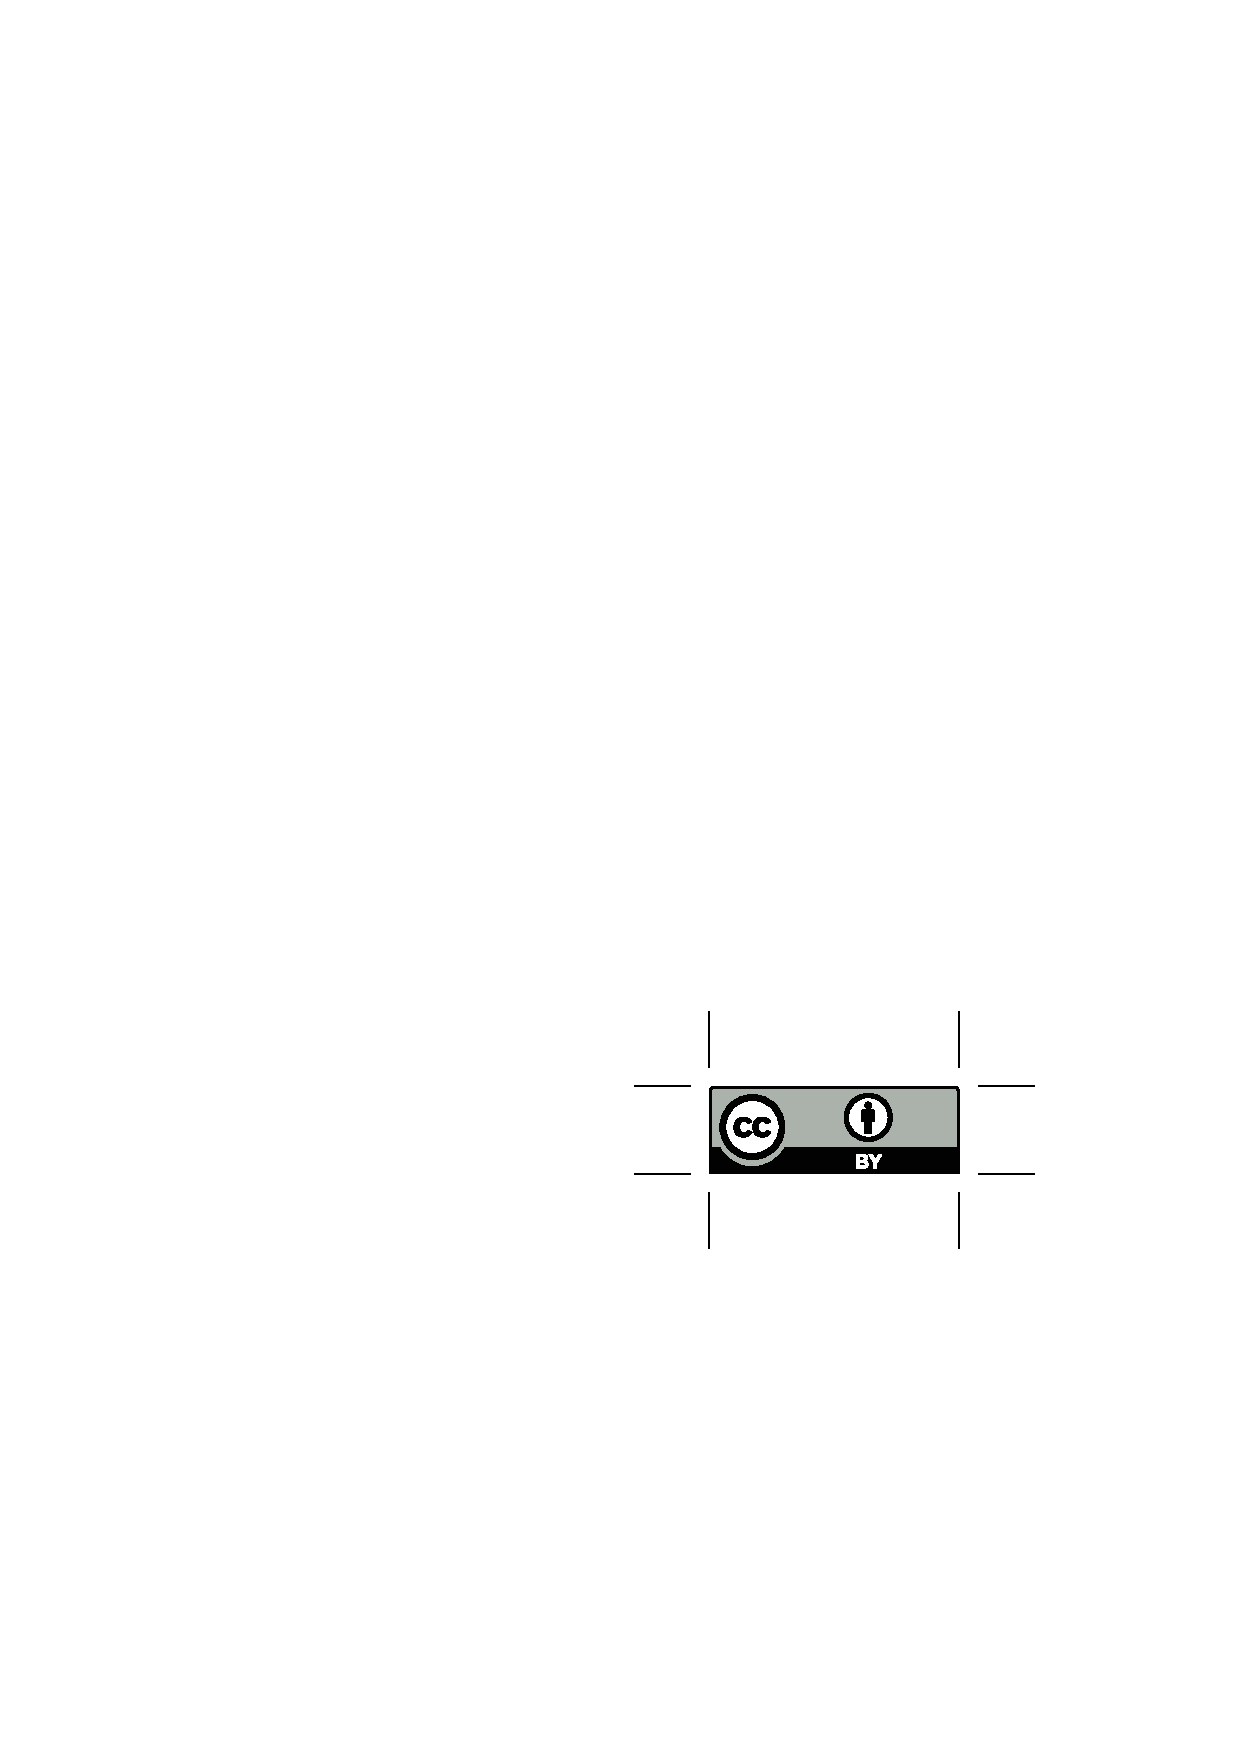
\includegraphics[width=0.90\textwidth]{by}}
  \end{minipage}\hfill
  \begin{minipage}{0.8\columnwidth}
   \href{https://creativecommons.org/licenses/by/4.0/}{This work is licensed under a Creative Commons Attribution International 4.0 License.}
  \end{minipage}
  \vspace{5pt}
}
\makeatother

\setcopyright{ifaamas}
\acmConference[AAMAS '25]{Proc.\@ of the 24th International Conference
on Autonomous Agents and Multiagent Systems (AAMAS 2025)}{May 19 -- 23, 2025}
{Detroit, Michigan, USA}{Y.~Vorobeychik, S.~Das, A.~Nowé  (eds.)}
\copyrightyear{2025}
\acmYear{2025}
\acmDOI{}
\acmPrice{}
\acmISBN{}

%%% ----- End macro definitions -----

\begin{document}

\pagestyle{fancy}
\fancyhead{}

\twocolumn

%%% The next command prints the information defined in the preamble.


\section{Safe Pareto Improvements in Belief-Conditioned Program Games}\label{sec:bcpg}

%%% PREVIOUS VERSION OF INTRO (commented out; superseded by the version below, which restructures (\ref{intro:bf})/(\ref{intro:scb}) around the in-fact/expectation distinction)
% Here, we extend the program game framework from~\citet{digiovanni2024safe} to a setting that doesn't assume simultaneous play. In particular, in this extension:
% \begin{enumerate}
%     \item Players' programs can condition on each other's \termemph{beliefs} about their counterpart, in addition to each other's source code.
%     \item We model two ways in which each player's beliefs can vary with the players' choices of programs:
%     \begin{enumerate}
%     %... Our framework also lets us speak of what each player's beliefs would have been in worlds where their counterpart used a different program; this is a separate, counterfactual form of belief-program dependence that we will need both to handle non-simultaneous game structures and to formulate the counterfactual checks on full strategies in~\S\ref{sub:pifi}.
%     \end{enumerate}
% \end{enumerate}
% We call this setting a \termemph{belief-conditioned program game}.
%
% %These extensions are motivated as follows.
% The motivation for the first item is that, if players are AI systems, their beliefs about counterparts may be explicitly represented (e.g., as parameters of a learned model) in a way that is amenable to verification~\citep{foerster2019bayesian, wang2022model}.
% Allowing programs to condition on such beliefs
% enables a player to check properties of the reasoning process that gave rise to their counterpart's program, not just the program itself.
% We will see that this is useful for the construction of subjectively rational SPIs.
% Motivating the two sub-items together, each player may reason that their choice of program gives them evidence about, or influences, what their counterpart believes about them. (If players agree on a model of this “influence'' on each other, the two sub-items are just two expressions of this same model --- but we won't assume the players agree on such a model, in general.)
% %This is natural if players engage in Stackelberg-like reasoning~\citep{colman1998stackelberg} or evidential decision theory~\citep{ahmed2021evidential}, and it is especially plausible when players simulate each other using mutual transparency of their code.
% %\footnote{More broadly, in settings where agents reason acausally about each other --- e.g., because each believes the other runs a sufficiently reliable simulation of them --- neither agent may be able to agree with the other on a specific ``logical order'' of moves. This motivates a symmetric model, rather than the sequential model of~\citet[Sec.~4]{digiovanni2023sufficient}, in which one player is designated as the first mover.}
% The remainder of this section formalizes these ideas.

%%%%% POTENTIAL REWRITE
% Here, we extend the program game framework from~\citet{digiovanni2024safe} to a setting that doesn't assume simultaneous play. (As in that paper, we'll start with the case of two players.)
% These extensions are motivated by two observations.

% \paragraph{Belief verification and subjective rationality of SPIs.} ...

% First, in 
% ... if players are AI systems, their beliefs about counterparts may be explicitly represented (e.g., as parameters of a learned model) in a way that is amenable to verification~\citep{foerster2019bayesian, wang2022model}.
% Allowing programs to condition on such beliefs
% enables a player to check properties of the reasoning process that gave rise to their counterpart's program, not just the program itself.
% We will see that this is useful for the construction of subjectively rational SPIs.


% In particular, in this extension:
% \begin{enumerate}
%     \item Players' programs can condition on each other's \emph{beliefs} about their counterpart, in addition to each other's source code. \label{intro:belcond}
%     \item  Players' programs and their beliefs about each other are interdependent in two ways:
%     \begin{enumerate}
%         \item Each player's beliefs about their counterpart are a \textit{function} of the counterpart's choice of program.
%         %\ ... A player's distribution over their counterpart's beliefs and program may depend on the counterpart's program --- possibly counterfactually, since the player needn't actually observe the counterpart's program. 
%         \label{intro:bf}
%         %         \item Each player might expect their choice to influence their counterpart:\ the player's distribution over the counterpart's program (and beliefs) might be conditioned on the program they themselves submit.
%         \item The beliefs in~(\ref{intro:bf}) are 
%         %represented as 
%         a distribution over possible counterparts \textit{conditional} on the program the player themselves submits. 
%         %--- capturing that the player may expect their own choice to be evidentially correlated with, or to influence, their counterpart's beliefs and program.
%         \label{intro:scb}
%         %         \item Each player's beliefs might be influenced by their counterpart's choice:\ the \textit{way in which the player forms the conditional distribution} in the previous item might depend, counterfactually, on their counterpart's program.
%     \end{enumerate}
% \end{enumerate}
% We call this setting a \emph{belief-conditioned program game}.

% % \paragraph{Motivation.}
% % Part~(\ref{intro:belcond}) of this extension captures the idea that,
% % if players are AI systems, their beliefs about counterparts may be explicitly represented (e.g., as parameters of a learned model) in a way that is amenable to verification~\citep{foerster2019bayesian, wang2022model}.
% % Allowing programs to condition on such beliefs
% % enables a player to check properties of the reasoning process that gave rise to their counterpart's program, not just the program itself.
% % We will see that this is useful for the construction of subjectively rational SPIs.

% Parts~(\ref{intro:bf}) and~(\ref{intro:scb}) capture how, under non-simultaneous play, each player's beliefs about their counterpart
% depend on \textit{both} players' programs:\ Due to sequential play or non-causal correlations between players' programs and beliefs,
% a player's beliefs might be influenced by their counterpart's program choice (part~(\ref{intro:bf})). In turn, each player may condition their beliefs
% about their counterpart on their own program choice, 
% because they expect to influence their counterpart's beliefs or decisions (part~(\ref{intro:scb})).
% (We'll see below
% that it helps to conceptually separate the functional dependence in~(\ref{intro:bf})
% from the conditioning in~(\ref{intro:scb}).)

Here, we extend the program game framework from~\citet{digiovanni2024safe} to a setting that doesn't assume simultaneous play. (As in that paper, we'll start with the case of two players.) In particular, in this extension:
\begin{enumerate}
    \item Players' programs can condition on each other's \emph{beliefs} about their counterpart, in addition to each other's program's source code. \label{intro:belcond}
    \item  Players' programs and their beliefs about each other are interdependent in two ways:
    \begin{enumerate}
        \item Each player's beliefs about their counterpart are a \textit{function} of the counterpart's choice of program.
        %\ ... A player's distribution over their counterpart's beliefs and program may depend on the counterpart's program --- possibly counterfactually, since the player needn't actually observe the counterpart's program. 
        \label{intro:bf}
        %         \item Each player might expect their choice to influence their counterpart:\ the player's distribution over the counterpart's program (and beliefs) might be conditioned on the program they themselves submit.
        \item The beliefs in~(\ref{intro:bf}) are 
        %represented as 
        a distribution over possible counterparts \textit{conditional} on the player's own program. 
        %--- capturing that the player may expect their own choice to be evidentially correlated with, or to influence, their counterpart's beliefs and program.
        \label{intro:scb}
        %         \item Each player's beliefs might be influenced by their counterpart's choice:\ the \textit{way in which the player forms the conditional distribution} in the previous item might depend, counterfactually, on their counterpart's program.
    \end{enumerate}
\end{enumerate}
We call this setting a \emph{belief-conditioned program game}.

\paragraph{Motivation.}
Part~(\ref{intro:belcond}) of this extension captures the idea that, if players are AI systems, their beliefs about counterparts may be explicitly represented (e.g., as parameters of a learned model) in a way that is amenable to verification~\citep{foerster2019bayesian, wang2022model}.
When programs can condition on such beliefs,
players can check properties of the reasoning process that produced their counterpart's program, not just the program itself.
%% A bit opaque at this stage:
This will help us construct subjectively rational SPIs in non-simultaneous settings.

Parts~(\ref{intro:bf}) and~(\ref{intro:scb}) capture how, under non-simultaneous play, each player's beliefs about their counterpart
depend on \textit{both} players' programs:\ Due to sequential play, or non-causal correlations between players' programs and beliefs,
a player's beliefs might be influenced by their counterpart's program choice (part~(\ref{intro:bf})). In turn, each player may condition their beliefs
about their counterpart on their own program choice, 
because they expect to influence their counterpart's beliefs or decisions (part~(\ref{intro:scb})).
(We'll see below
that it helps to conceptually separate the functional dependence in~(\ref{intro:bf})
from the conditioning in~(\ref{intro:scb}).)

%Part~(\ref{intro:bf}) captures how, when the game isn't strictly simultaneous, 
%players' beliefs about each other's programs
%can in fact
%depend on those programs --- e.g., due to sequential play or non-causal correlations between players' programs.


%Part~(\ref{intro:scb}) captures a separate effect: a player may reason that their own choice of program is evidentially correlated with, or causally influences, what their counterpart believes about them --- making the player's beliefs depend on their own choice as well.
%absent strict simultaneity, the counterpart's program --- or counterfactual versions of it, relevant to the conditions on full strategies in~\S\ref{sub:pifi} --- plausibly shifts what a player believes about them.
%The motivation for~(\ref{intro:scb}) is that each player may further reason that their own choice of program gives them evidence about, or influences, what their counterpart believes about them.

%The remainder of this section formalizes these ideas.


\subsection{Setup: Base Games and Simultaneous Program Games}\label{sub:basegame}

We begin by recalling the relevant definitions from~\citet{digiovanni2024safe}.
Two players $i=1,2$ will play a base game of complete information $\game = (\allact = \actspaceone \times \actspacetwo, (\payone, \paytwo))$,
where $\actspacei$ is the set of possible actions for player~$i$ and $\payi(\fullact)$ is player~$i$'s payoff when the action profile $\fullact = (\actone, \acttwo)$ is played.
Write $\fullpay(\fullact) = (\payone(\fullact), \paytwo(\fullact))$.
%%% might put this back in, but not relevant for now bc not dealing with PMM
%and refer to the set of payoff profiles attainable by some $\fullact \in \allact$ as the \termemph{feasible set}.
Throughout, we use the index~$j$ for the player $j \neq i$.
For payoff profiles~$\mathbf{x}$ and~$\mathbf{y}$, write $\mathbf{x} \succeq \mathbf{y}$ if $x_i \geq y_i$ for all~$i$, and $\mathbf{x} \succ \mathbf{y}$ if $x_i > y_i$ for all~$i$.
%Assume the action sets are continuous; this is practically without loss of generality, because programs can use correlated randomization~\citep{kalai2010commitment}.

A \termemph{simultaneous program game} is a game with the following structure: Each player~$i$'s strategy is a program $\progi \in \progspacei$ --- a computable function from $\progspacej$ to $\actspacei$ --- that maps the other player's program to an action in~$\game$.\footnote{\ We restrict to deterministic programs for ease of exposition; the extension to probabilistic programs is straightforward~\citep{kalai2010commitment}.}
Once all the programs are simultaneously submitted, the induced action profile $\fullact(\fullprog) = (\progone(\progtwo), \progtwo(\progone))$ is played in~$\game$, and player~$i$'s payoff is $\progpayi(\fullprog) = \payi(\fullact(\fullprog))$.


\subsection{Belief-Conditioned Programs and Conditional Beliefs}\label{sub:bcprog}

We now extend simultaneous program games along two dimensions.

\paragraph{Belief-conditioned programs.}
In belief-conditioned program games, each player~$i$'s program takes as input not only the other player's program~$\progj$, but also the other player's \textit{belief function} (defined below).
This allows player~$i$'s action to depend on the reasoning process that informed player~$j$'s choice of program. 
%(which, as we'll see, is essential for making SPIs subjectively rational in non-simultaneous games).
%verifying properties such as participation independence.
%~\citep[Sec.~4.3]{digiovanni2023sufficient}.

Specifically, let:
\begin{itemize}
    \item $\scbspacei$ be the space of $i$'s self-conditional beliefs (defined momentarily);
    \item $\beliefspacei$ be a set of belief functions
    %$\beta_i: \bcprogspacej \to \scbspacei$
    (defined momentarily); and
    \item $\bcprogspacei$ be a set of computable functions from $\bcprogspacej \times \beliefspacej$ to~$\actspacei$.
\end{itemize}
The spaces $\scbspacei, \beliefspacei, \bcprogspacei$ ($i = 1,2$) are defined in terms of each other; this mutual recursion is the standard higher-order belief structure from epistemic game theory.\footnote{ \ Formally, these spaces are defined as a fixed point. Existence follows from the universal type space construction~\citep{mertens1985formulation, brandenburger1993hierarchies}. In practice, if players' higher-order reasoning terminates at finite depth, the spaces are well-defined without this machinery.}

We assume that all programs in $\bcprogspacei$ halt against all programs in~$\bcprogspacej$ (as is standard in the program game literature; see, e.g., \citet{tennenholtz2004program, oesterheld2019robust}).
We denote the \termemph{belief-conditioned program game} as $\game(\allbcprog)$, where $\allbcprog = \bcprogspaceone \times \bcprogspacetwo$.

\paragraph{Belief functions and self-conditional beliefs.}
%In simultaneous program games, players' beliefs about each other's programs are fixed, independent of either player's choice of program.
To allow for non-simultaneous program choice,
we let player~$i$'s beliefs depend on both~$j$'s program and on~$i$'s own program.
%However, for non-simultaneous games,
%(or when $i$ may verify counterfactual properties of~$j$'s reasoning)
%we want to capture 
%how~$i$'s beliefs (counterfactually) depend on~$j$'s choice of program.
%--- the counterfactual dependence flagged in the introduction.
%Separately, the player may reason that their own choice of program is evidentially correlated with, or causally influences, their counterpart's beliefs and program choice --- making the conditional dependence on the player's own program non-trivial.
%\footnote{\ This conditional dependence is about how~$i$'s distribution shifts \textit{across} different choices of~$\progi$, not the spread of~$i$'s beliefs at a fixed~$\progi$. For example, if a player in a simultaneous game of Chicken is merely uncertain whether~$j$'s program will swerve, that uncertainty lives in the support of~$\tau_i(\cdot \mid \progi)$ at a fixed~$\progi$ --- it doesn't itself make~$\tau_i$ vary across~$\progi$.}
We model
these two kinds of dependence
with different formal objects --- respectively, \textit{belief functions} and \textit{self-conditional beliefs} ---
to highlight an epistemic asymmetry:\ On one hand, player~$i$ might not observe their counterpart's program~$\progj$ at the time of choice, so~$i$'s beliefs depend on~$\progj$ via some exogenous function (rather than via conditioning). On the other hand, they do know their own program $\progi$, so they can directly condition their beliefs on $\progi$. 

First, a \termemph{belief function} $\beta_i \in \beliefspacei$ maps each (counterfactual) program of~$j$ to
%a collection of
self-conditional beliefs:
$$
\beta_i : \bcprogspacej \to \scbspacei.
$$
%This function captures how~$j$'s choice of program affects~$i$'s beliefs.
%The value $\beta_i(\progj)$ is the self-conditional beliefs~$i$ would hold \emph{in the world where~$j$'s actual program is~$\progj$}.
A few clarifications about~$\beta_i$ :
\begin{enumerate}
    \item \emph{The form of the function~$\beta_i$ reflects the game's structure.}
    In simultaneous program games, every~$\progj$ maps to the same self-conditional beliefs $\beta_i(\progj)$.
    In other game structures (e.g., sequential), $\beta_i$ may depend non-trivially on~$\progj$. In particular, the forms of the belief functions determine which player, if any, is the “first mover''.    
    \item \emph{$\beta_i$ is not a posterior-update rule.}
    $\beta_i(\progj)$ encodes ``the self-conditional beliefs~$i$ would have in the world where~$j$'s actual program is~$\progj$'', \emph{not} ``$\tau_i$ after~$i$ observes~$\progj$''.
    %In particular,~$i$ does not necessarily observe~$j$'s program at the time~$i$ chooses a program (e.g., the game might be simultaneous).
    This will be important when, in~\S\ref{sub:pifi}, we consider how players might want to condition their programs' outputs on properties of each other's \textit{counterfactual} program choice.
    %%% revisit phrasing below
%    \item \emph{The counterfactual reading is essential for participation and foreknowledge independence.}
%    As we'll formalize in~\S\ref{sub:pifi}, checking whether~$i$'s program satisfies these conditions involves asking what~$i$ would've chosen if~$j$'s program were, e.g., $j$'s
    %%% "default" not yet defined
    %% Easiest fix: add one sentence introducing "default" at first use ("the program i would have used absent any SPI mechanism"), or forward-reference to the renegotiation section. I'd lean introducing it informally on first use to keep this section self-contained.
%    default --- and this requires the structural mapping~$\beta_i$, not a Bayesian update.
\end{enumerate}

Second, \termemph{self-conditional beliefs} $\tau_i \in \scbspacei$ give~$i$'s joint distribution over~$j$'s program~$\progj$ and belief function~$\beta_j$, \textit{conditional} on~$i$ choosing program~$\progi$:\footnote{\ Formally, $\tau_i$ is a stochastic kernel; we reserve the word ``function'' for the structurally different object~$\beta_i$ above.
\\ \textit{(\textbf{TO DO:} say something about how for FDT or the like, the conditional can be replaced with a counterfactual)}}
%how~$i$'s beliefs about~$j$'s type (program~$\progj$ \emph{and} belief function~$\beta_j$) depend on~$i$'s own program choice:
$$
\tau_i(\cdot \mid \progi) \in \Delta(\bcprogspacej \times \beliefspacej).
$$
%That is, conditional on~$i$ choosing program~$\progi$, $\tau_i$ gives~$i$'s joint distribution over pairs $(\progj, \beta_j)$.

(Why a distribution over~$j$'s program \textit{and} belief function?
Because, first, in a belief-conditioned program game player~$i$'s expected payoff
%from some program
depends on~$j$'s possible belief functions.
%% MAKE CLEARER %%
% Second, we can't necessarily assume that~$i$ deduces~$j$'s program by computing the
% subjectively optimal program with respect to~$\beta_j$.
To do so,~$i$ would need to know~$j$'s expected payoff from each candidate program, which depends on~$i$'s \textit{own} subjectively optimal program. This kind of cross-agent best-response recursion is what subjective equilibrium is supposed to relax.)
%This is because~$i$ can only do this if~$i$ knows what \textit{their own} subjectively optimal program is.)
% [Claude:]
% Second, we can't simply assume that i deduces j's program by computing j's subjectively optimal program given β_j. To do so, i would need to know j's expected payoff from each candidate program — which depends on i's own program — so i would already need to know i's own subjectively optimal program. This kind of cross-agent best-response recursion is what subjective equilibrium is supposed to relax.

%Jointness lets us state subjective equilibrium without imposing cross-agent consistency at the level of the formalism: $i$'s beliefs about~$j$'s program need not match the program~$j$ would in fact play under~$\beta_j$.
%%% phrasing above very unclear
%Cross-agent consistency can be imposed later as an explicit belief assumption when needed, analogous to the ``no-punishment'' assumption of~\citet{digiovanni2024safe}.\footnote{\ Two distinct pairs $(\beta_j, \progj)$ and $(\hat{\beta}_j, \hat{p}_j)$ may correspond to distinct types of counterpart --- e.g., different reasoning processes generating different (or the same) programs. Because programs in~$\bcprogspacei$ take~$\beta_j$ as an input in addition to~$\progj$, they can distinguish such cases.}

See Fig.~\ref{fig:bcpg} for a summary of the model. Both $\beta_i$ and $\tau_i$ are primitives of the model. Before submitting their program, each player~$i$ only knows their \textit{own} $\beta_i$ and $\tau_i$.
But after both programs are submitted, each~$\progi$ can read~$\beta_j$.
%The two interdependencies introduced in~\S\ref{sec:bcpg} are captured directly by the framework's primitives.
%Interdependency~(\ref{intro:bf}) --- beliefs as a counterfactual function of the counterpart's program --- is captured by belief functions $\beta_i$ and $\beta_j$: each $\beta_k$ specifies what player~$k$'s beliefs would be across counterfactual programs of the counterpart.
%Interdependency~(\ref{intro:scb}) --- beliefs as a conditional distribution given the player's own program --- is captured by self-conditional beliefs $\tau_i$ and $\tau_j$: each $\tau_k(\cdot \mid p_k)$ is player~$k$'s distribution over the counterpart given $k$ has committed to $p_k$ (which is what matters for modeling player~$k$'s program choice, since~$k$ conditions on what~$k$ picks).
%We take both players' belief functions and self-conditional beliefs as primitives of the model.

\paragraph{Relationship to the standard setting.} The setup reduces to the standard program game of~\citet{digiovanni2024safe} under these conditions:  
$\tau_i(\cdot \mid \progi)$ is independent of~$\progi$; $\beta_i$ is constant in~$\progj$; and programs do not condition on belief functions (i.e., $\bcprogspacei$ reduces to the standard program space $\progspacei$).

\begin{figure}[t]
\centering
\begin{tikzpicture}[
  node distance=1.3cm and 2.0cm,
  every node/.style={font=\small},
  arr/.style={->, >=stealth, thick}
]
  % Player 1
  \node (Beta1) {$\beta_1$};
  \node[right=3cm of Beta1] (Beta2) {$\beta_2$};
  \node[below=of Beta1] (B1) {$\tau_1$};
  \node[below=of Beta2] (B2) {$\tau_2$};
  \node[below=of B1] (p1) {$\progone$};
  \node[below=of B2] (p2) {$\progtwo$};
  \node[below=of p1] (a1) {$\actone$};
  \node[below=of p2] (a2) {$\acttwo$};

  % Belief function to self-conditional beliefs
  \draw[arr] (Beta1) -- (B1);
  \draw[arr] (Beta2) -- (B2);

  % Self-conditional beliefs to own program (via EU max)
  \draw[arr] (B1) -- (p1);
  \draw[arr] (B2) -- (p2);

  % Programs to own actions
  \draw[arr] (p1) -- (a1);
  \draw[arr] (p2) -- (a2);

  % Cross arrows: each program's output depends on counterpart's program
  \draw[arr] (p2) -- (a1);
  \draw[arr] (p1) -- (a2);

  % Belief functions are inputs to counterpart's program (dashed)
  \draw[arr, dashed] (Beta2) -- (a1);
  \draw[arr, dashed] (Beta1) -- (a2);

  % Counterpart's program feeds into self-conditional beliefs (dotted)
  \draw[arr, densely dotted] (p2) -- (B1);
  \draw[arr, densely dotted] (p1) -- (B2);

  % Labels
  \node[above=0.15cm of Beta1] {\footnotesize Player 1};
  \node[above=0.15cm of Beta2] {\footnotesize Player 2};
\end{tikzpicture}
\caption{Functional dependencies in a belief-conditioned program game.
Solid arrows show the main causal chain: player~$i$'s belief function~$\beta_i$ determines~$i$'s self-conditional beliefs~$\tau_i$,
%(combined with~$j$'s actual program --- dotted arrow),
which determines~$i$'s program~$\progi$ via EU maximization. In turn, both players' programs determine~$i$'s action.
Dashed arrows indicate that~$i$'s action also depends on~$j$'s belief function~$\beta_j$, which is an input to~$i$'s program.
Dotted arrows indicate that~$\tau_i$ is determined by~$\beta_i$ evaluated at~$j$'s actual program.}
\label{fig:bcpg}
\end{figure}


% We model this by endowing each player~$i$ with a \termemph{conditional belief function} $\beliefi \in \beliefspacei$, where
% $$
% \beliefi(\cdot \mid \progi) \in \Delta(\beliefspacej \times \brspacej)
% $$
% gives player~$i$'s beliefs about player~$j$'s conditional belief function \emph{and} best-response function, conditional on player~$i$ choosing program~$\progi$.
% The spaces $\beliefspacei$ and $\beliefspacej$ are thus defined in terms of each other --- $\beliefi$ maps into distributions over $\beliefspacej \times \brspacej$, and vice versa --- but this mutual recursion is the standard higher-order belief structure familiar from epistemic game theory.\footnote{Formally, the spaces $(\beliefspacei, \beliefspacej)$ are defined as a fixed point of the mapping that sends each player's belief space to the set of conditional distributions over the other's. The existence of such spaces follows from the universal type space construction~\citep{mertens1985formulation, brandenburger1993hierarchies}. In practice, if players' higher-order reasoning terminates at finite depth, the spaces are well-defined without this machinery.}
% %That is, $\beliefi$ is an ``epistemic algorithm'' that takes $i$'s own program choice as input and outputs beliefs about the epistemic algorithm and decision procedure of~$j$.

% Crucially, $\beliefi$ does not directly model how~$i$ updates on information about~$j$'s program; rather, it captures how~$i$'s own choice gives~$i$ evidence about~$j$'s reasoning.
% Two related but distinct questions are worth separating:
% (1)~how~$i$'s beliefs are \emph{in fact} influenced by~$j$'s program, and
% (2)~how~$j$ \emph{expects}~$i$'s beliefs to be influenced by~$j$'s program.
% For the purposes of modeling~$j$'s incentives, only~(2) matters, and it is captured by~$j$'s conditional belief function~$\beliefj$.
% Question~(1) is determined by the structure of the game,
% e.g., whether it's sequential.
% %--- e.g., in a sequential game where~$i$ first observes some information about~$\progj$, one could stipulate a mapping from~$j$'s program to~$i$'s conditional belief function, or impose consistency constraints requiring~$i$'s beliefs to be compatible with what~$i$ has observed.
% Here,
% we'll just take both players' conditional belief functions as primitives of the model.

% Note that~$i$'s uncertainty is over the pair $(\beliefj, \brj)$ --- $j$'s conditional belief function and best-response function --- rather than over~$j$'s program directly or over~$j$'s ``bottom-line'' beliefs $\beliefj(\cdot \mid \progj)$ at some particular~$\progj$.
% There are two reasons for this.
% First, programs in~$\bcprogspacei$ take~$\beliefj$ and~$\brj$ as input, so they can inspect counterfactual properties of~$j$'s reasoning --- e.g., what program~$j$ would have chosen under different beliefs about~$i$ --- that are not determined by~$j$'s program alone.\footnote{Two distinct pairs $(\beliefj, \brj)$ and $(\hat{\beliefj}, \hat{\brj})$ may yield the same program $\brj(\beliefj) = \hat{\brj}(\hat{\beliefj})$ yet have different counterfactual properties, e.g., they may produce different programs under alternative beliefs about~$i$. Programs in~$\bcprogspacei$ can distinguish these cases.}
% Second, $j$'s best-response function $\brj$ takes~$j$'s entire conditional belief function as input --- since $j$ optimizes over~$\progj$ accounting for how $\beliefj(\cdot \mid \progj)$ varies with~$\progj$ --- so the pair $(\beliefj, \brj)$ is the natural ``type'' for player~$j$.

% Player~$i$'s beliefs about player~$j$'s \emph{program} are then derived: for each $(\beliefj, \brj)$ in the support of $\beliefi(\cdot \mid \progi)$, player~$j$'s program is $\brj(\beliefj)$.
% Thus $\beliefi$ induces a distribution over $\bcprogspacej$ via the pushforward of $(\beliefj, \brj) \mapsto \brj(\beliefj)$, but the primitive object of uncertainty is the pair $(\beliefj, \brj)$.

% In the special case where $\beliefi(\cdot \mid \progi) = \beliefi(\cdot \mid \progi')$ for all~$\progi, \progi' \in \bcprogspacei$, this reduces to an unconditional belief, recovering the standard program game setting of~\citet{digiovanni2024safe} (once belief-conditioning of programs is also dropped).
% But in general, $\beliefi$ allows player~$i$'s beliefs to vary with their own program choice, capturing the possibility that~$i$ believes their counterpart partially predicts~$i$'s program or that $i$'s decision is evidentially correlated with~$j$'s.

% \begin{figure}[t]
% \centering
% \begin{tikzpicture}[
%   node distance=1.3cm and 2.0cm,
%   every node/.style={font=\small},
%   arr/.style={->, >=stealth, thick}
% ]
%   % Player 1
%   \node (B1) {$\beliefone$};
%   \node[right=3cm of B1] (B2) {$\belieftwo$};
%   \node[below=of B1] (br1) {$\brone$};
%   \node[below=of B2] (br2) {$\brtwo$};
%   \node[below=of br1] (p1) {$\progone$};
%   \node[below=of br2] (p2) {$\progtwo$};
%   \node[below=of p1] (a1) {$\actone$};
%   \node[below=of p2] (a2) {$\acttwo$};

%   % Beliefs to BR functions
%   \draw[arr] (B1) -- (br1);
%   \draw[arr] (B2) -- (br2);

%   % BR functions to programs
%   \draw[arr] (br1) -- (p1);
%   \draw[arr] (br2) -- (p2);

%   % Programs to own actions
%   \draw[arr] (p1) -- (a1);
%   \draw[arr] (p2) -- (a2);

%   % Cross arrows: each program's output depends on counterpart's program
%   \draw[arr] (p2) to[bend left=15] (a1);
%   \draw[arr] (p1) to[bend right=15] (a2);

%   % Beliefs and BR are inputs to counterpart's program (dashed)
%   \draw[arr, dashed] (B2) to[bend left=30] (a1);
%   \draw[arr, dashed] (br2) to[bend left=20] (a1);
%   \draw[arr, dashed] (B1) to[bend right=30] (a2);
%   \draw[arr, dashed] (br1) to[bend right=20] (a2);

%   % Conditional beliefs depend on own program (dotted)
%   \draw[arr, densely dotted] (p1) to[bend left=50] (B1);
%   \draw[arr, densely dotted] (p2) to[bend right=50] (B2);

%   % Labels
%   \node[above=0.15cm of B1] {\footnotesize Player 1};
%   \node[above=0.15cm of B2] {\footnotesize Player 2};
% \end{tikzpicture}
% \caption{Functional dependencies in a belief-conditioned program game with conditional beliefs.
% Solid arrows show the causal chain for each player: conditional beliefs feed the best-response function, which selects a program, which determines an action.
% Dashed arrows indicate that each player's action also depends on their counterpart's conditional belief function and best-response function, which are inputs to the player's program.
% Dotted arrows indicate that each player's conditional beliefs about the counterpart's belief function and best-response function may depend on the player's own choice of program.}
% \label{fig:bcpg}
% \end{figure}


%\paragraph{Interpretation.}
%This framework is symmetric: both players have the same type of self-conditional beliefs and belief function, and neither is fixed as the ``first mover''.
%Which player moves first, if any, is determined by the belief functions.
%This contrasts with the sequential belief-conditioned program game of~\citet[Sec.~4.2]{digiovanni2023sufficient}, in which player~1 is assumed to move first and player~2 updates beliefs by partially predicting player~1's program.
% The present model can be viewed as a symmetric generalization of 
% a framework where one player chooses a program first, 
% applicable when both players reason that they have some influence over their counterpart's beliefs --- as may be the case when AI agents simulate each other and neither can agree on a definite logical order of moves.\footnote{\ The “player~1 moves first'' model 
% %of~\citet{digiovanni2023sufficient 
% is a special case. To recover it: $\beta_2(\progone)$ varies non-trivially with~$\progone$ (encoding player~2's observation of player~1's program), while $\beta_1$ is constant in~$\progtwo$ (player~1 has no observation). Likewise, player~1's self-conditional beliefs $\tau_1(\cdot \mid \progone)$ vary non-trivially with~$\progone$,
% capturing player~1's expectation that
% $(\beta_2, \progtwo)$ depends on their choice of~$\progone$; while~$\tau_2$ is constant in~$\progtwo$.}


\begin{example}[Partial observation in Chicken]
Consider a belief-conditioned program game where the base game is Chicken (Table~\ref{tab:chicken}).
%each player has actions $\actspacei = \{\text{Swerve}, \text{Dare}\}$, with the highest payoff to a unilateral driver, the middle payoff to mutual swerving, and the worst payoff to mutual driving.
Suppose player~2's program space is partitioned into two disjoint subsets: $\progspacetwo^{\text{H}}$ (\textit{hawkish} programs that mostly play Dare) and $\progspacetwo^{\text{D}}$ (\textit{dovish} programs that mostly play Swerve).
Before choosing their program, player~1 observes whether player~2 is hawkish or dovish.
Let $\progspacetwo^{\progtwo}$ be the subset in this partition containing player~2's chosen~$\progtwo$.
Then, player~1's belief function $\beta_1$ is such that
$\beta_1(\progtwo)$ puts positive probability only on programs in $\progspacetwo^{\progtwo}$.
%Let player~1's belief function~$\beta_1$ depend on~$\progtwo$ only through which side of this partition~$\progtwo$ lies on --- player~1 effectively observes whether player~2 is hawkish or dovish, but nothing finer.
Player~2 doesn't observe anything about player~1's program, so~$\beta_2$ is constant in~$\progone$.
%The game is non-simultaneous (player~1 has partial information about~$\progtwo$) without being strictly sequential (player~1 doesn't see~$\progtwo$ in full).
In this setting, player~2 might commit to a program~$\progtwo^{\text{H}} \in \progspacetwo^{\text{H}}$, anticipating that player~1 will (correctly) infer this and best-respond by swerving. So,~$\beta_2(\progone)(\cdot \mid \progtwo^{\text{H}})$ puts high probability on $\progone$ being dovish.
\label{ex:chicken}
\end{example}
%--- a strategic move not available under strict simultaneity.

\begin{table}
    \centering
    \caption{Payoff matrix for Chicken}
    \begin{tabular}{c|c|c|}
          \multicolumn{1}{c}{} & \multicolumn{1}{c}{Swerve} & \multicolumn{1}{c}{Dare}\\
     \cline{2-3}
      Swerve & $3, 3$ & $1, 4$ \\
        \cline{2-3}
      Dare & $4, 1$ & $0, 0$ \\
       \cline{2-3}
    \end{tabular}
    \label{tab:chicken}
\end{table}

\subsection{Payoffs, SPIs, and Subjective Equilibrium}\label{sub:outcomes}

Given a profile of programs $\fullprog = (\progone, \progtwo)$ and a profile of belief functions $\fullbf = (\beta_1, \beta_2)$, the action profile played in the base game is
$$
\fullact(\fullprog, \fullbf) = \bigl(\progone(\progtwo, \beta_2),\; \progtwo(\progone, \beta_1)\bigr).
$$
Player~$i$'s payoff is
$$
\progpayi^{\fullbf}(\fullprog) := \payi\bigl(\fullact(\fullprog, \fullbf)\bigr).
$$

\paragraph{SPIs for belief-conditioned program games.} We can then define SPIs in this new setting as follows, adapting Definition~2 of~\citet{digiovanni2024safe} to payoffs that depend on both program and belief-function profiles.

\begin{definition}[SPI for a belief-conditioned program game]
\label{def:bcpg-spi}
For a belief-conditioned program game $\game(\allbcprog)$,
let $\fullfs : \allbcprog \to {\allbcprog}'$ be a function of program profiles, written $\fullfs(\fullprog) = (\fsprogone(\progone), \fsprogtwo(\progtwo))$, for some joint program space ${\allbcprog}'$.\footnote{\ As with $\allbcprog$, we assume programs in ${\allbcprog}'$ halt against each other and take the counterpart's program and belief function as inputs.}
Then~$\fullfs$ is an \textbf{SPI for $\game(\allbcprog)$} if:
\begin{itemize}
    \item for all program profiles $\fullprog$ and belief function profiles $\fullbf$,
    $$\fullprogpay^{\fullbf}(\fullfs(\fullprog)) \succeq \fullprogpay^{\fullbf}(\fullprog);$$
    \item and for some $(\fullprog, \fullbf)$, there is some $i'$ such that
    $\progpayip^{\fullbf}(\fullfs(\fullprog)) > \progpayip^{\fullbf}(\fullprog)$.
\end{itemize}
\end{definition}

As in the simultaneous setting, the transformation acts only on programs. But the Pareto improvement must hold \emph{regardless} of the players' belief function profile~$\fullbf$.
%A belief-conditioned program can still \emph{read} the counterpart's belief function at runtime (e.g., to verify counterfactual properties of the counterpart's reasoning); the requirement is only that the improvement is robust across belief-function profiles.

\paragraph{Subjective equilibrium and miscoordination.} Each player~$i$ chooses their program to maximize expected utility under their 
%\emph{actual} 
self-conditional beliefs $\tau_i$.
This $\tau_i$ is determined by~$\beta_i$ evaluated at the counterpart's actual~$\progj$. (So, we can define subjective equilibrium in terms of just $(\fullprog, \fullbf)$.) But, recall, we do not assume player~$i$ \textit{knows} the actual~$\progj$, only the output~$\tau_i$.
%Because~$\tau_i$ is itself determined by~$\beta_i$ evaluated at the actual~$\progj$, subjective equilibrium amounts to a fixed-point condition on the profile~$(\fullprog, \fullbf)$.

\begin{definition}[Subjective equilibrium of belief-conditioned program game]
\label{def:bcpg-subjeq}
Let $\fulleq = (\eqprogone, \eqprogtwo)$ and $\fullbf = (\beta_1, \beta_2)$ be profiles of programs and belief functions, respectively, in $\game(\allbcprog)$.
And define $\eqscbi := \beta_i(\eqprogj)$, that is,
player~$i$'s self-conditional beliefs under $\fulleq$ and $\fullbf$.
We say $(\fulleq, \fullbf)$ is a \textbf{subjective equilibrium} of $\game(\allbcprog)$ if, for each~$i$,
$$
\eqprogi \in \arg\max_{\progi \in \bcprogspacei}
\mathbb{E}_{(\progj', \beta_j') \sim \eqscbi(\cdot \mid \progi)} \; \payi\bigl(\progi(\progj', \beta_j'),\, \progj'(\progi, \beta_i)\bigr).
$$
\end{definition}

In this definition:
\begin{itemize}
    %\item The expectation is with respect to player~$i$'s actual self-conditional beliefs $\eqscbi$, i.e.,~$\beta_i$ evaluated at~$j$'s actual (equilibrium) program.
    %This yields~$\tau_i = \beta_i(\eqprogj)$, $i$'s actual self-conditional beliefs.
    \item The expectation is over pairs~$(\progj', \beta_j') \sim \eqscbi(\cdot \mid \progi)$, i.e., $i$'s joint uncertainty about~$j$'s program and belief function, conditional on~$i$'s own program choice~$\progi$.
    \item For each realization~$(\progj', \beta_j')$, the payoff is computed by running~$\progi$ and~$\progj'$ against each other, passing in~$\beta_j'$ and~$\beta_i$ respectively as the belief function inputs. Crucially, no best-response operator is invoked: $\progj'$ is drawn directly from~$i$'s beliefs.
    This sidesteps the need to define player~$i$'s subjective expected utility in terms of information
    about~$\eqprogj$ (which player~$i$ realistically wouldn't have).
%    sidestepping any cross-agent best-response recursion.
\end{itemize}

As in~\citet{digiovanni2024safe}, subjective equilibrium is a weak solution concept.
Our results will be correspondingly strong: we will construct strategies that are preferred for \emph{any} self-conditional beliefs satisfying certain assumptions, and are thus used in every subjective equilibrium associated with those beliefs. Under the same conditions discussed in~\S\ref{sub:bcprog}, Definition~\ref{def:bcpg-subjeq} reduces to the standard notion of subjective equilibrium from~\citet{digiovanni2024safe}.

The base games of interest remain bargaining problems, in which players can miscoordinate in subjective equilibrium if they are sufficiently confident their counterparts will play favorably to them~\citep[Example~1]{digiovanni2024safe}.
Such miscoordination is possible even in belief-conditioned program games, for the same reasons as in the standard setting: players' self-conditional beliefs are underdetermined by their evidence, and may lead each player to adopt an aggressive program in the hope of exploiting a cautious counterpart.

\paragraph{The role of belief functions and self-conditional beliefs.}
The two objects introduced in \S\ref{sub:bcprog} create new considerations for the analysis of SPIs.
In~\citet{digiovanni2024safe}, simultaneous play ensures that each player's choice of program does not affect their counterpart's choice.
So in that setting, the main obstacle to subjective rationality of SPIs is the response of a \emph{fixed} counterpart program to an SPI-transformed program.
%(cf.~the ``consistent defaults'' condition).
With self-conditional beliefs, player~$i$ must additionally account for the risk that~$j$ might \emph{choose} a less favorable program, depending on whether~$i$ chooses to use an SPI.
%causes their counterpart to \termemph{choose} a less favorable program --- even under simultaneous play --- because the player believes their counterpart's beliefs (and hence best response) are influenced by the player's own decision.
%This is the symmetric analog of the sequential-play obstacle discussed in~\citet[Sec.~4.1]{digiovanni2023sufficient}.
In the subsequent sections, we show \textit{(\textbf{TO DO})} that belief-conditioned programs can address this risk, by allowing each player~$i$ to verify whether~$j$'s chosen program would have been different had~$i$ opted out of SPIs.
%\termemph{participation independence} of their counterpart's program --- specifically, by inspecting~$\beta_j$ and
%%% rephrase
%checking that counterfactuals computed via~$\beta_j$ leave~$j$'s program input to the SPI unchanged regardless of~$i$'s participation (\S\ref{sub:pifi}).


\subsection{Participation Independence and Foreknowledge Independence}\label{sub:pifi}

%%% rephrase
An SPI in isolation is just a transformation; whether it is subjectively rational depends on the programs it is applied to. We refer to a program profile $\fullprog \in \allbcprog$ to which an SPI~$\fullfs$ is applied as the \termemph{input strategies} for~$\fullfs$, and to $\fullfs(\fullprog)_i$ as player~$i$'s SPI-transformed program. We now define two conditions on input strategies that govern when SPIs are subjectively rational, depending on the game structure.

Participation independence (PI) and foreknowledge independence (FI) formalize two counterfactual checks on input strategies:
%%% need to be careful with phrasing here; we'll return to this
in each, we ask whether player~$i$ would still select their input strategy~$\progi$, given
some counterfactual that refers to the possibility “$j$ uses~$\progj$ rather than the SPI-transformed~$\fullfs(\fullprog)_j$”. They differ in what the counterfactual counterfactually changes: PI counterfactually changes~$j$'s \emph{program}; FI counterfactually changes~$i$'s \emph{beliefs} about~$j$. As the definitions below show, the formal conditions don't reference~$\fullfs$ itself: PI and FI are properties of the pair~$(\fullprog, \fullbf)$ alone. 
%The SPI is the conceptual occasion for asking the counterfactual, but it doesn't enter the math.

\begin{definition}[Participation-independent input strategies]
\label{def:pi}
Given a belief-function profile $\fullbf$, the \textbf{participation-independent counterfactual choice} of player~$i$ given $(\progj, \fullbf)$ is
$$
\progi^{\text{PI}}(\progj, \fullbf) \;\in\; \arg\max_{\hat{\progi} \in \bcprogspacei} \; \mathbb{E}_{(\progj', \beta_j') \sim \beta_i(\progj)(\cdot \mid \hat{\progi})} \; \payi\bigl(\hat{\progi}(\progj', \beta_j'),\, \progj'(\hat{\progi}, \beta_i)\bigr).
$$
The input strategies $\fullprog$ are \textbf{participation-independent} (relative to~$\fullbf$) if $\progi \in \progi^{\text{PI}}(\progj, \fullbf)$ for each~$i$.
\end{definition}

\begin{definition}[Foreknowledge-independent input strategies]
\label{def:fi}
Abusing notation, given a belief-function profile $\fullbf$, let
$\beta_i(\progj)(\,\cdot\, \mid \hat{\progi},\, \progj' = \progj)$ denote the conditional distribution of~$\beta_j'$ under the joint self-conditional beliefs $\beta_i(\progj)(\,\cdot\, \mid \hat{\progi})$, given the event that~$j$'s program equals~$\progj$.
Then, the \textbf{foreknowledge-independent counterfactual choice} of player~$i$ given $(\progj, \fullbf)$ is
$$
\progi^{\text{FI}}(\progj, \fullbf) \;\in\; \arg\max_{\hat{\progi} \in \bcprogspacei} \; \mathbb{E}_{\beta_j' \sim \beta_i(\progj)(\,\cdot\, \mid \hat{\progi},\, \progj' = \progj)} \; \payi\bigl(\hat{\progi}(\progj, \beta_j'),\, \progj(\hat{\progi}, \beta_i)\bigr).
$$
The input strategies $\fullprog$ are \textbf{foreknowledge-independent} (relative to $\fullbf$) if $\progi \in \progi^{\text{FI}}(\progj, \fullbf)$ for each~$i$.
\end{definition}

The two definitions differ in how the counterfactual enters the argmax:
\begin{enumerate}
    \item In PI, the counterfactual “$j$ uses~$\progj$”
    enters the argmax only via the \textit{input to~$\beta_i$}.
    %    ... is defined in terms of~$i$'s self-conditional beliefs in the counterfactual where~$j$ used the program~$\progj$, that is, $\beta_i(\progj)$.
    But the definition of PI uses the full joint $\beta_i(\progj)(\cdot \mid \hat{\progi})$ over $(\progj', \beta_j')$: $i$'s uncertainty about both~$j$'s program and~$j$'s belief function is preserved, and $i$'s actual~$\beta_i$ still governs how that uncertainty varies with possible programs~$\hat{\progi}$ that~$i$ could choose.
    \item In FI, the counterfactual also enters via \textit{an event that~$i$'s self-conditional beliefs are conditioned on}. That is, FI conditions the joint distribution on the event $\{\progj' = \progj\}$: $i$'s marginal uncertainty over~$j$'s program is collapsed to a point mass on~$\progj$.
\end{enumerate}
%but uncertainty over~$\beta_j$ is retained (as the conditional distribution given that event).

\paragraph{Sanity check (simultaneous case).}
When the game structure is simultaneous, $\beta_i(\progj)$ is constant in~$\progj$, so it equals~$i$'s actual self-conditional beliefs~$\tau_i$ regardless of~$\progj$. The PI condition then reduces to: for each~$i$,
$$
\progi \in \arg\max_{\hat{\progi} \in \bcprogspacei} \; \mathbb{E}_{(\progj', \beta_j') \sim \tau_i(\cdot \mid \hat{\progi})} \; \payi\bigl(\hat{\progi}(\progj', \beta_j'),\, \progj'(\hat{\progi}, \beta_i)\bigr),
$$
which is exactly the subjective-equilibrium condition on~$\progi$ under~$\tau_i$ (Definition~\ref{def:bcpg-subjeq}, with $\fullprog$ in the role of~$\fulleq$). In other words, under simultaneous play, the input strategies~$\fullprog$ are participation-independent iff $\fullprog$ itself constitutes a subjective equilibrium ---
%%% not quite, that paper doesn't refer to PI at all
recovering the observation of~\citet{digiovanni2024safe} that PI holds automatically when input strategies are in simultaneous-play equilibrium.
FI remains non-trivial in this case: conditioning~$\tau_i$'s joint distribution on $\{\progj' = \progj\}$ (point mass on~$\progj$, conditional belief over~$\beta_j$) can yield a different best response from PI's unconditioned expectation.


\subsection{[WIP] Participation-Independent Renegotiation}\label{sub:pireneg}

We now construct an SPI for belief-conditioned program games --- which we'll call \termemph{participation-independent (PI) renegotiation} --- by adapting the renegotiation construction of~\citet[Sec.~3.2]{digiovanni2024safe} to the belief-conditioned setting. PI-conditional renegotiation programs only engage when the input strategies they wrap satisfy participation independence (Definition~\ref{def:pi}).

\paragraph{Renegotiation programs in BCPG}
Recall that a \termemph{renegotiation function}~$\smreneg : \allact \to \allact$, as defined in~\citet[Sec.~3.2]{digiovanni2024safe}, maps action profiles to weakly Pareto-improved profiles, with strict improvement on at least one profile. The corresponding \termemph{renegotiation programs} of~\citet[Algorithm~1]{digiovanni2024safe} carry $\smrenegi$ and a \termemph{default program}~$\defprogi$ as parameters; against any counterpart program that is also a renegotiation program with a renegotiation function that agrees with~$\smrenegi$ on the default action profile, the renegotiation program plays its part of the renegotiated outcome, and otherwise plays its default's action.

We adapt this construction to BCPG by allowing each program to additionally read the counterpart's belief function~$\beta_j$, in line with the BCPG program signature; the extra input is needed below for the PI check.

\paragraph{PI-conditional renegotiation}
A \termemph{PI-conditional renegotiation program} is a BCPG renegotiation program that additionally checks, at runtime, that the counterpart's default program $\defprogj$ is participation-independent given the joint default profile $\deffullprog = (\defprogi, \defprogj)$ under the actual belief-function profile~$\fullbf$. Formally, the program engages iff
$$\defprogj \in \progj^{\text{PI}}(\defprogi, \fullbf).$$
Player~$i$'s program has access to all four objects $(\defprogi, \beta_i, \defprogj, \beta_j)$ at runtime --- $\defprogi$ and $\beta_i$ from $i$'s own state, $\beta_j$ from the input directly, and $\defprogj$ recovered from the structure of~$\progj$ (since~$\progj$ is verified to be a PI-conditional renegotiation program with parameter~$\defprogj$). So the check is well-typed.\footnote{\ The computational cost is dominated by the $\arg\max$ over $\bcprogspacej$ used to define $\progj^{\text{PI}}$. We don't address this here; structural / syntactic verification of $\defprogj$'s PI is a sound but incomplete substitute.}

Algorithm~\ref{alg:bcpg-pi-renegotiation} gives the full procedure. Let $\bcpirenegspacei(\smrenegi)$ be the set of all such programs for player~$i$, parameterized by~$\smrenegi$ and a default program $\defprogi \in \bcprogspacei \setminus \bcpirenegspacei(\smrenegi)$ (the disjoint-set requirement avoids circular self-reference, as in~\citet[Sec.~3.2]{digiovanni2024safe}). Note that the definition of Algorithm~\ref{alg:bcpg-pi-renegotiation} doesn't require its \textit{own} default program to be PI.

\begin{algorithm}
\caption{PI-conditional renegotiation program $\progi \in \bcpirenegspacei(\smrenegi)$, for some default $\defprogi$}
\label{alg:bcpg-pi-renegotiation}
\begin{algorithmic}[1]
\Require Counterpart program $\progj$, counterpart belief function $\beta_j$
\If{$\progj \in \bcpirenegspacej(\smrenegj)$ for some $\smrenegj \in \fullrenegspace$}
    \Comment{$\progj$ is also a PI-conditional renegotiation program}
    %\State Let $\defprogj$ be the default program of~$\progj$.
    \If{$\defprogj \in \progj^{\text{PI}}(\defprogi, \fullbf)$}
        \Comment{Counterpart's default is PI}
        \State $\deffullact \leftarrow \fullact(\deffullprog, \fullbf)$
        \If{$\smrenegi(\deffullact) = \smrenegj(\deffullact)$}
            \State \Return $\renii(\deffullact)$
            \Comment{Play renegotiated action}
        \Else
            \State \Return $\defacti$
            \Comment{Play default's action against counterpart's default}
        \EndIf
    \Else
        \State \Return $\defprogi(\progj, \beta_j)$
        \Comment{Counterpart's default not PI}
    \EndIf
\Else
    \State \Return $\defprogi(\progj, \beta_j)$
    \Comment{Counterpart not a PI-conditional renegotiation program}
\EndIf
\end{algorithmic}
\end{algorithm}

%Algorithm~\ref{alg:bcpg-pi-renegotiation} doesn't separately verify that $i$'s own default is PI under the actual~$\fullbf$; we treat this as a usage requirement, captured in the hypothesis of the proposition below.

% \paragraph{The PI-conditional renegotiation transformation as an SPI}
% Following Proposition~1 of~\citet{digiovanni2024safe}, we now show that the PI-conditional renegotiation construction yields an SPI for $\game(\allbcprog)$.

% \begin{proposition}
% \label{prop:pi-spi}
% Let~$\smreneg$ be a renegotiation function. For~$i = 1, 2$, define $\fsprogi: \bcprogspacei \to \bcpirenegspacei(\smreneg)$ such that, for each~$\progi \in \bcprogspacei$, $\fsprogi(\progi)$ has the form of Algorithm~\ref{alg:bcpg-pi-renegotiation} with $\defprog{\fsprogi(\progi)} = \progi$. Then,
% $$
% \fullfs : \fullprog \mapsto \bigl(\fsprogone(\progone),\; \fsprogtwo(\progtwo)\bigr)
% $$
% is an SPI for $\game(\allbcprog)$.
% \end{proposition}
% \begin{proof}
% \textit{Weak Pareto improvement (for all $(\fullprog, \fullbf)$).} When both players play their transformed programs, the outer structural identification step of Algorithm~\ref{alg:bcpg-pi-renegotiation} succeeds (both are PI-conditional renegotiation programs using the same~$\smreneg$). The PI check on the counterpart's default $\defprogj = \progj$ then either (i)~passes, in which case both players play the renegotiated action profile $\smreneg(\fullact(\fullprog, \fullbf))$, which weakly Pareto-improves $\fullact(\fullprog, \fullbf)$ by definition of a renegotiation function; or (ii)~fails, in which case both players play~$\fullact(\fullprog, \fullbf)$ itself. Either way, $\fullprogpay^{\fullbf}(\fullfs(\fullprog)) \succeq \fullprogpay^{\fullbf}(\fullprog)$.

% \textit{Strict improvement for some $(\fullprog, \fullbf)$.} Take any $(\fullprog, \fullbf)$ for which the input strategies~$\fullprog$ are participation-independent under~$\fullbf$ (Definition~\ref{def:pi}) and~$\smreneg$ strictly Pareto-improves $\fullact(\fullprog, \fullbf)$ for some player. The PI check then passes by hypothesis, and~$\smreneg(\fullact(\fullprog, \fullbf))$ is strictly preferred to $\fullact(\fullprog, \fullbf)$ by some player, so the strict-improvement clause of the SPI definition (Definition~\ref{def:bcpg-spi}) is satisfied.
% \end{proof}


\begin{table}[!htbp]
    \caption{Key notation introduced in this section}
    \label{tab:notation-bcpg}
    \begin{tabular}{rl}\toprule
        \textit{Symbol} & \textit{Description (page introduced)} \\ \midrule
        $\bcprogspacei$ & set of belief-conditioned programs for player~$i$ \\
        & (computable functions from $\bcprogspacej \times \beliefspacej$ \\
        & to~$\actspacei$) (\pageref{sub:bcprog}) \\
        $\game(\allbcprog)$ & belief-conditioned program game with joint \\
        & program space $\allbcprog = \bcprogspaceone \times \bcprogspacetwo$ \\
        & (\pageref{sub:bcprog}) \\
        $\beliefspacei$, $\beta_i$ & set of belief functions for player~$i$, and an \\
        & element thereof: $\beta_i: \bcprogspacej \to \scbspacei$ maps each \\
        & (counterfactual)~$\progj$ to a self-conditional belief \\
        & (\pageref{sub:bcprog}) \\
        $\scbspacei$, $\tau_i$ & set of player~$i$'s self-conditional beliefs, and \\
        & an element thereof: a stochastic kernel \\
        & $\tau_i(\cdot \mid \progi) \in \Delta(\bcprogspacej \times \beliefspacej)$ giving~$i$'s joint \\
        & distribution over $(\progj, \beta_j)$ given~$i$'s own~$\progi$ \\
        & (\pageref{sub:bcprog}) \\
        $\fullbf$ & profile of belief functions $(\beta_1, \beta_2)$ \\
        & (\pageref{sub:outcomes}) \\
        $\fullact(\fullprog, \fullbf)$ & action profile played in the base game given \\
        & program profile~$\fullprog$ and belief-function profile~$\fullbf$ \\
        & (\pageref{sub:outcomes}) \\
        $\progpayi^{\fullbf}(\fullprog)$ & player~$i$'s payoff $\payi(\fullact(\fullprog, \fullbf))$ \\
        & (\pageref{sub:outcomes}) \\
        $\fullfs$ & SPI transformation acting on program profiles, \\
        & with components $\fsprogi$ acting on each player's \\
        & program (\pageref{sub:outcomes}) \\
        $\eqscbi$ & player~$i$'s equilibrium self-conditional beliefs, \\
        & $\beta_i(\eqprogj)$ (\pageref{sub:outcomes}) \\
        $\progi^{\text{PI}}(\progj, \fullbf)$ & participation-independent counterfactual choice \\
        & for player~$i$ given $(\progj, \fullbf)$ (\pageref{sub:pifi}) \\
        $\progi^{\text{FI}}(\progj, \fullbf)$ & foreknowledge-independent counterfactual choice \\
        & for player~$i$ given $(\progj, \fullbf)$ (\pageref{sub:pifi}) \\
        \bottomrule
    \end{tabular}
\end{table}

\bibliography{main}


\end{document}

%%% ----- Notation summary (for reference) -----
% 
% Symbol                   Description
% -------                  -----------
% B_i \in \beliefspacei    Conditional belief function for player i:
%                            maps i's own program to beliefs about
%                            j's conditional belief function
% B_i(.|\progi) \in           Player i's beliefs about B_j,
%   \Delta(B_j)              conditional on i choosing \progi
% P^BC_i                   Belief-conditioned program space for player i:
%                            set of functions from 
%                            P^BC_j x \beliefspacej to A_i
% U_i^{B}(p)               Player i's payoff given program profile p
%                            and conditional belief profile B
%
%%% ----- End notation summary -----